\newpage
\section{Setting up your M2T workspace}
\genHeader

Nowadays, \emph{no one} really writes a complex parser completely by hand. Although this is sometimes still necessary\footnote{Some languages are syntactically
quite challenging.} most parsers can be whipped up pretty quickly using context-free \emph{string grammars}\footnote{For simple cases, \emph{regular
expressions} can also be used.} typically in EBNF\footnote{Extended Backus-Naur Form}.
ANTLR~\cite{ANTLR} is a tool that can generate a parser from a compact EBNF specification for a host of target programming languages, including Java.
Although ANTLR might not be the most efficient or powerful parser generator out there, it is open-source, well documented and supported, and allows for a
pragmatic and quite elegant \emph{fallback} to Java when things get nasty and we have to resort to some dirty tricks.


% --------------------------------------------------------------------------------------------------------------------------------------------------------
% 	Does there need to be a 'fresh start section?' i.e, do we need to briefly explain/tell where to look for info? Does user need to download anything from
% previous parts?
% \subsection{A fresh start}
% --------------------------------------------------------------------------------------------------------------------------------------------------------


The first step is preparing an Eclipse workspace according to our suggested workflow.

% \jumpDual{}{}

\newpage
\hypertarget{initialize vis}{}
\subsection{First steps}
\visHeader

\begin{itemize}

\item[$\blacktriangleright$] From your Eclipse workspace, open the \texttt{Dict\-ion\-ary.eap} file in Enterprise Architect (EA). The project browser should
closely resemble Fig.~\ref{ea:mocaTagged}. As you can see, the project is already populated with \texttt{MocaTree} and other built-in metamodels
in the \texttt{eMoflon Languages} working set.

\vspace{0.5cm}

\begin{figure}[htpb]
\begin{center}
  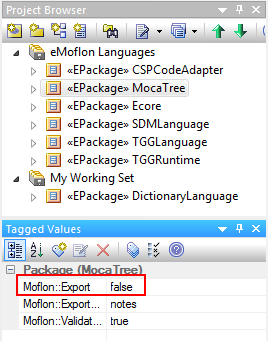
\includegraphics[width=0.4\textwidth]{ea_mocaTaggedValues}
  \caption{\texttt{MocaTree} is one of eMoflons' internal metamodels}
  \label{ea:mocaTagged}
\end{center}
\end{figure}

\end{itemize}

\vspace{-0.5cm}

If you inspect the tagged values\footnote{The ``Tagged Values'' window can be opened by going to ``View/Tagged Values'' or by hovering over the \texttt{Tagged
Values} tab immediately to the right of the project browser.} for these built-in languages, you'll notice that the \texttt{MocaTree} package has the
\texttt{Moflon::Export} value set to \texttt{false}. This ensures that the package is \emph{ignored} when exporting. As with all such standard metamodels (e.g.,
Ecore or our SDM metamodel) the \texttt{MocaTree} package in EA should be regarded as read-only, required only in the EA project so that SDMs/TGGs can refer to
the classes defined in the package.

\begin{itemize}

\item[$\blacktriangleright$] Despite \texttt{DictionaryLanguage} being contained in a different working set than \texttt{MocaTree}, the two
metamodels are contained within the same EA project (EAP) which means you are able to create a new TGG using them both. Add a new package to \texttt{My
Working Set} named \texttt{Dict\-ion\-ary\-Code\-Adap\-ter}.

\item[$\blacktriangleright$] Select the package and add a new TGG schema diagram as depicted in Fig.~\ref{ea:newTGGDiagram}. In the next dialogue window,
set the source project as \texttt{MocaTree}, and the target project as \texttt{Dict\-ion\-ary\-Lang\-uage}.

\begin{figure}[h!]
\begin{center}
  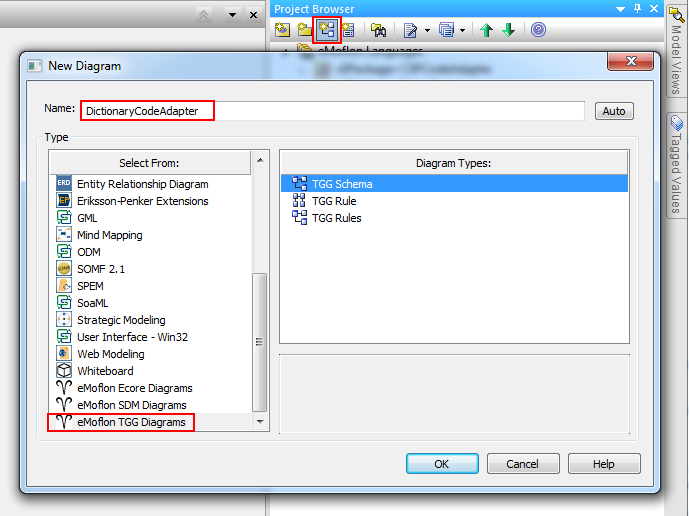
\includegraphics[width=0.9\textwidth]{ea_adapterTGGDiagram}
  \caption{Create a new TGG schema diagram}
  \label{ea:newTGGDiagram}
\end{center}
\end{figure}

\item[$\blacktriangleright$] For the moment, add a single correspondence type to the new diagram now active in the editor (the TGG \texttt{schema}) between
\texttt{Folder} and \texttt{Library}. Remember, you can get the classes by drag-and-dropping each element into the diagram, then quick-creating a new
\texttt{TGG Correspondence Type} between them.\footnote{For details on the correspondence metamodel and how to create types, refer to Part IV, Section 3.} Your diagram
should come to resemble Fig.~\ref{ea:firstCorrType}.

\vspace{0.5cm}

\begin{figure}[htpb]
\begin{center}
  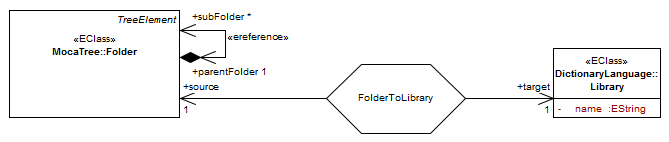
\includegraphics[width=\textwidth]{ea_firstAdapterCorrespondence}
  \caption{The first correspondence type for the transformation}
  \label{ea:firstCorrType}
\end{center}
\end{figure}

\newpage

\item[$\blacktriangleright$] Your complete project browser should now resemble Fig.~\ref{ea:TGGProjBrow}, where \texttt{Dict\-ion\-ary\-Code\-Adap\-ter} is now
explicitly listed as a \texttt{TGGSchemaPackage}.

\vspace{0.5cm}

\begin{figure}[htpb]
\begin{center}
  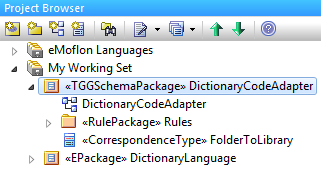
\includegraphics[width=0.5\textwidth]{ea_TGGProjectBrowser}
  \caption{A fully prepared TGG project}
  \label{ea:TGGProjBrow}
\end{center}
\end{figure}

\item[$\blacktriangleright$] Validate and export your file via the eMoflon control panel,\footnote{Activate via ``Extensions/Add-in Windows''} then switch
back to Eclipse and refresh the package explorer. A new \texttt{Dict\-ion\-ary\-Code\-Adap\-ter} project should appear in \texttt{My Working Set}.

\jumpSingle{subSec:setupParser}

\end{itemize}


\newpage
\hypertarget{M2TSettingUp tex}{}
\subsection{Initializing the project}
\texHeader

{\bf SELF:: update download so it includes a constraint file for \texttt{Dictionary}}
\begin{figure}[htbp]
\begin{center}
  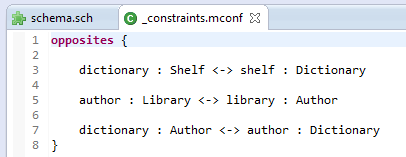
\includegraphics[width=0.7\textwidth]{eclipse_DOWNLOADUPDATE}
  \caption{SELF SELF}
\end{center}
\end{figure}

\begin{enumerate}

\item[$\blacktriangleright$] Your expanded \texttt{DictionaryLanguage} metamodel MOSL structure should resemble FIG. (starting point) You'll notice that it is
accessing the \emph{Moca} framework by importing the \texttt{MocaTree} in \texttt{\_imports.mconf}. (Explain, no screenshot?)

\item[$\blacktriangleright$] Right click on \texttt{MyWorkingSet} folder and create a new TGG. source: MocaTree. Target: DictionaryLanguage. FIG

\begin{figure}[htbp]
\begin{center}
  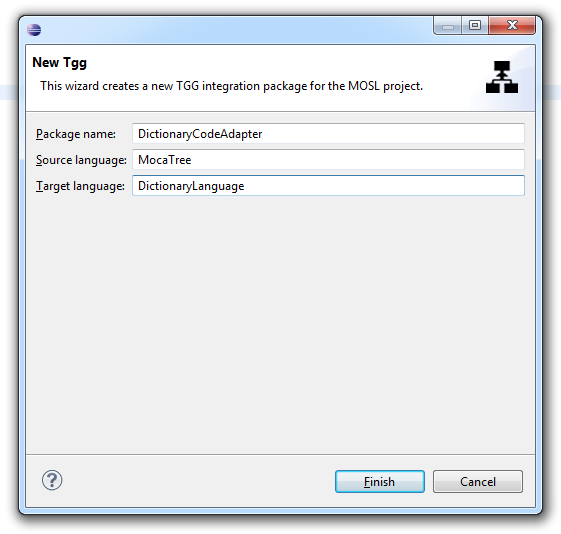
\includegraphics[width=0.9\textwidth]{eclipse_dictionaryCodeAdapterTGGProject}
  \caption{create tgg}
  \label{eclipse:newTGGProject}
\end{center}
\end{figure}


\item[$\blacktriangleright$] Before saving and building, initialize the correct generated code type by establishing the schema below (default is..)

\begin{figure}[htbp]
\begin{center}
  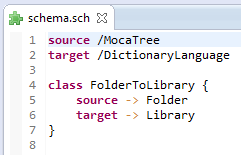
\includegraphics[width=0.5\textwidth]{eclipse_schemaStart}
  \caption{first rule}
  \label{eclipse:firstSchema}
\end{center}
\end{figure}

\item[$\blacktriangleright$] Save and build your project! Confirm a generated project was created in the \texttt{MyWorkingSet} node, and carry on!

\end{enumerate}

